\chapter{LODでの公開機構}
本章ではLODでの公開機構について述べる.

\section{スキーマとURI}

\subsection{RDFスキーマ定義}
サービスのユーザーを表すUserスキーマを\ref{table:user_scheme},
ミッションを表すMissionスキーマを\ref{table:mission_scheme},
ミッションに属するタスクを表すTaskスキーマを\ref{table:task_scheme},
タスクに対するコメントを表すCommentスキーマを\ref{table:comment_scheme}に示す.

\begin{table}[t]
 \caption{Userスキーマ}
 \begin{center}
	 \begin{tabular}{ | c | c | c | } \hline
	    Property & Type & Description \\ \hline \hline
			image & Image & プロフィール画像 \\ \hline
			name & Text & 名前 \\ \hline
	 \end{tabular}
	 \label{table:user_scheme}
 \end{center}
\end{table}

\begin{table}[t]
 \caption{Missionスキーマ}
 \begin{center}
	 \begin{tabular}{ | c | c | c | } \hline
	    Property & Type & Description \\ \hline \hline
			title & Text & タイトル \\ \hline
			description & Text & 概要 \\ \hline
			creator & User & 作成者 \\ \hline
			created & DateTime & 作成日時 \\ \hline
			modified & DateTime & 編集日時 \\ \hline
	 \end{tabular}
	 \label{table:mission_scheme}
 \end{center}
\end{table}

\begin{table}[t]
 \caption{Taskスキーマ}
 \begin{center}
	 \begin{tabular}{ | c | c | c | } \hline
	    Property & Type & Description \\ \hline \hline
			title & Text & タイトル \\ \hline
			description & Text & 概要 \\ \hline
			missionOf & Mission & 所属しているミッション \\ \hline
			leader & User & リーダー \\ \hline
			collaborator & User & コラボレータ \\ \hline
			status & Text & 進捗状況 \\ \hline
			link & URL & リンク \\ \hline
			comment & Comment & コメント \\ \hline
			subTaskOf & Task & 親タスク \\ \hline
			created & DateTime & 作成日時 \\ \hline
			modified & DateTime & 編集日時 \\ \hline
	 \end{tabular}
	 \label{table:task_scheme}
 \end{center}
\end{table}

\begin{table}[t]
 \caption{Commentスキーマ}
 \begin{center}
	 \begin{tabular}{ | c | c | c | } \hline
	    Property & Type & Description \\ \hline \hline
			name & Text & 名前 \\ \hline
			message & Text & メッセージ本文 \\ \hline
			created & DateTime & 作成日時 \\ \hline
			modified & DateTime & 編集日時 \\ \hline
	 \end{tabular}
	 \label{table:comment_scheme}
 \end{center}
\end{table}

\subsection{URIエンドポイント}

\section{アクセス制御}
先に述べたように,ゴオルシェアではLinked Dataのアクセス権限を指定することができず,自動的にすべてのデータが誰でも閲覧できる状況にあった.
しかし研究室など限られた組織内で使うには,アクセス権限のあるユーザーのみが閲覧できる仕組みが必要である.
そこで現状では,アカウント単位でのアクセスコントロール機能があるRDFストアであるStardogを用いて,プロジェクトの段階に応じたアクセス制御機構を実装中である.
具体的には\ref{table:permission_table}に示すように,(1)プロジェクトが個人的な構想段階である初期場合,(2)組織内限定で共有される段階,(3)外部発表後に外部公開する段階,(4)オープンライセンスで公開し,組織横断的な協働を志向する段階,の4段階を想定し,各段階に応じたアクセス制御機構を想定している.
プロジェクトの段階が進んでいくにつれて,公開したいタスクが増えていくと考えられる.
ただし,より具体的な下層の葉に近いタスクは,段階が進んだとしても公開に適さない場合が多いと考えられる.
そこで,タスクツリーからユーザが公開したいタスクのみを部分的に選択できるようなインターフェースも必要となる.
このような公開箇所の選択機構についても,現在実装中である.

\begin{table}[t]
 \caption{アクセス権限}
 \begin{center}
	 \begin{tabular}{ | c || c | c | c | c | } \hline
		  & 個人的思想 & 組織内限定 & 外部公開 & LOD \\ \hline \hline
			Read & 作成者 & 組織内 & 誰でも & 誰でも \\ \hline
			Write & 作成者 & \shortstack{ 作成者 \\ メンバー } & \shortstack{ 作成者 \\ メンバー } & \shortstack{ 作成者 \\ メンバー } \\ \hline
			ライセンス & - & - & - & オープンライセンス \\ \hline
	 \end{tabular}
	 \label{table:permission_table}
 \end{center}
\end{table}

\section{実装手法}
ユーザーが投稿したミッションやタスクは,まずはメインデータベースであるMySQLに保存される.
個人的思想を選んだ場合は,そのユーザーに紐付いたStardogアカウントのみRead/WriteできるLODとして公開する.
組織内限定を選んだ場合は,その組織に紐付いたStardogアカウントのみReadでき,作成したユーザーに紐付いたStardogアカウントのみWriteできるLODとして公開する.
外部公開を選んだ場合は,作成したユーザーに紐付いたStardogアカウントのみWriteでき,誰でも自由にReadできるLODとして公開する.
LODを選んだ場合は,誰でも自由にRead/WriteできるLODとして公開する.

LODのRDFスキーマは前述したものを用い,MySQLのデータベースER図を\ref{img:system_model}に示す.

\begin{figure}[t]
	\begin{center}
		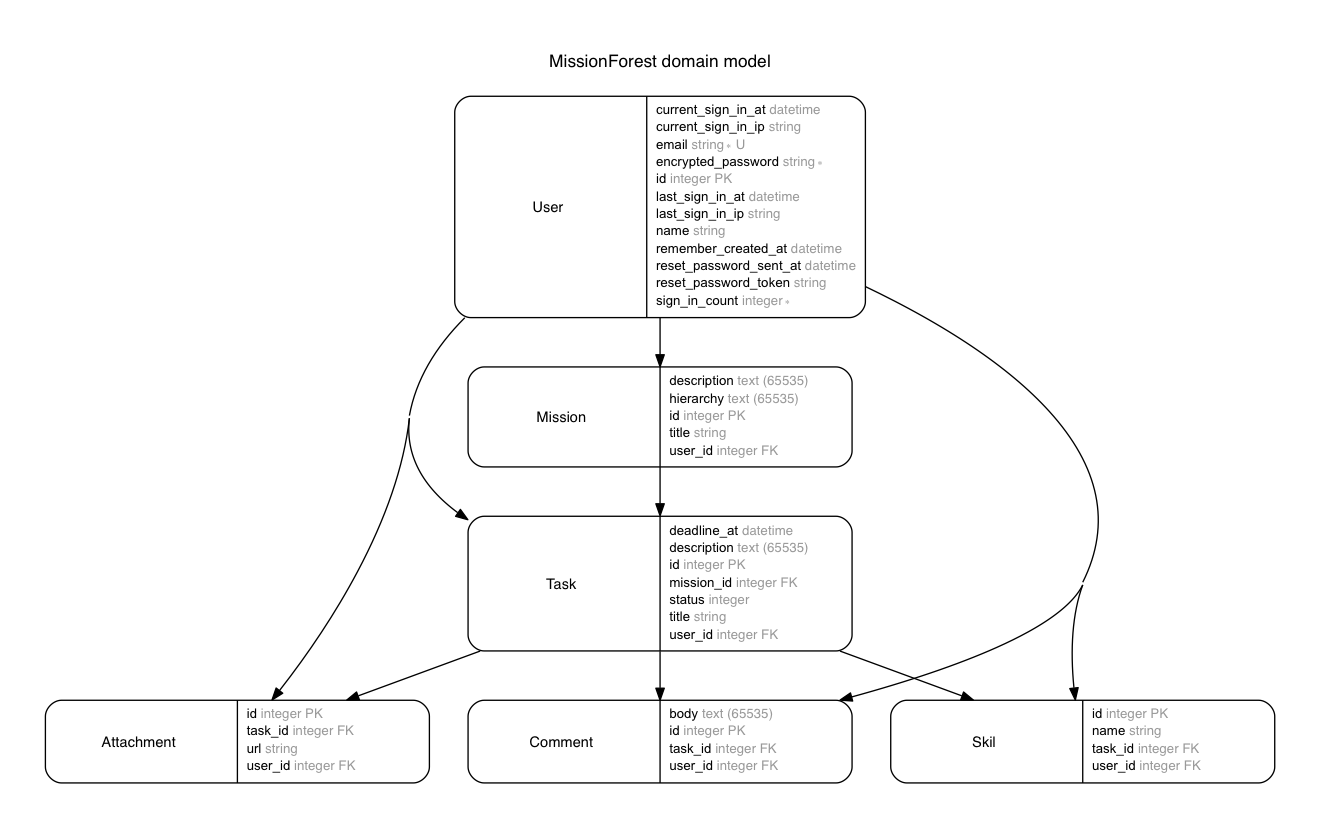
\includegraphics[width=0.9\linewidth]{assets/img/system_model.png}
		\caption{データベースER図}
		\label{img:system_model}
	\end{center}
\end{figure}
